\documentclass[border=10pt]{standalone}
\usepackage{tikz}
\usepackage[utf8]{inputenc}
\usepackage[T1]{fontenc}
\usetikzlibrary{patterns,arrows.meta,decorations.pathreplacing}

\begin{document}

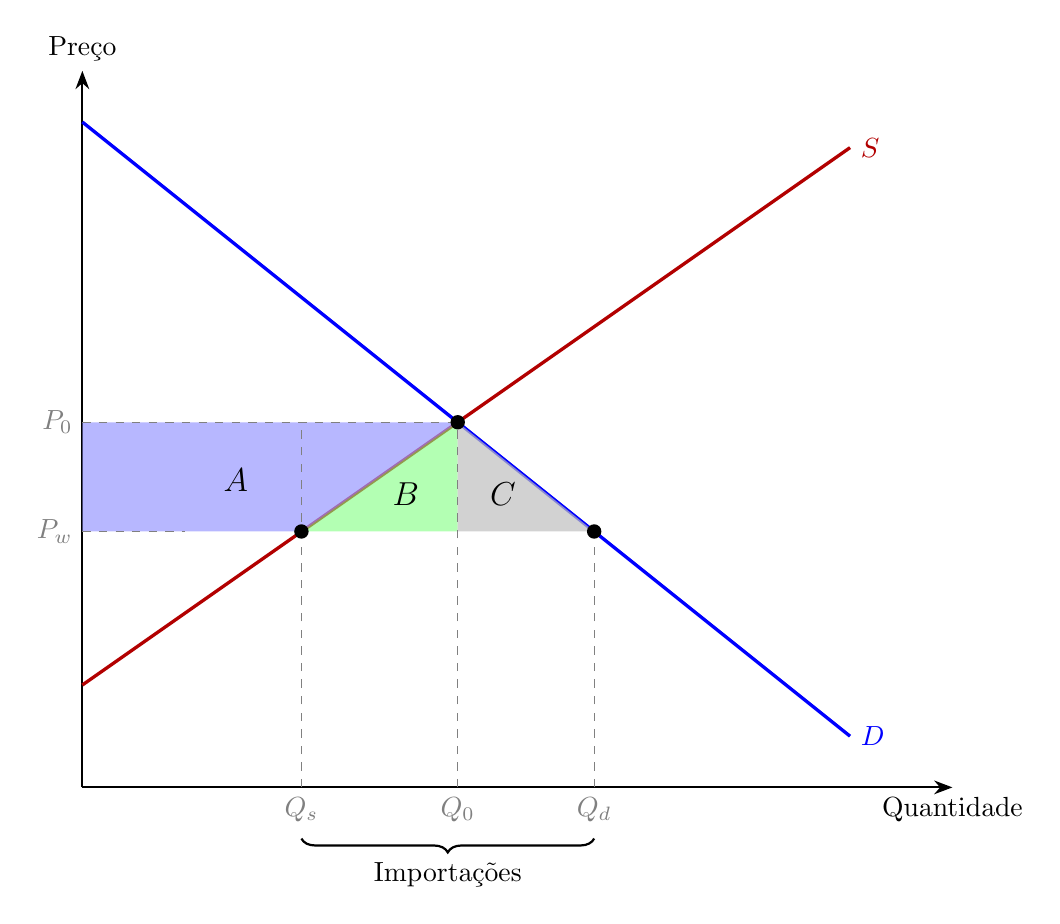
\begin{tikzpicture}[scale=1.3, >=Stealth]
    
    % Eixos
    \draw[thick,->] (0,0) -- (8.5,0) node[below] {Quantidade};
    \draw[thick,->] (0,0) -- (0,7) node[above] {Preço};
    
    % Curvas de oferta e demanda
    \draw[blue, very thick, domain=0:7.5] plot (\x, {6.5 - 0.8*\x}) node[right] {$D$};
    \draw[red!70!black, very thick, domain=0:7.5] plot (\x, {1.0 + 0.7*\x}) node[right] {$S$};
    
    % Coordenadas importantes
    % Equilíbrio: D = S => 6.5 - 0.8*x = 1.0 + 0.7*x => 5.5 = 1.5*x => x = 3.667, y = 3.567
    \def\Qeq{3.667}     % Quantidade de equilíbrio Q0
    \def\Peq{3.567}     % Preço de equilíbrio P0
    \def\Pw{2.5}        % Preço mundial (mais baixo)
    \def\Qs{2.14}       % Quantidade ofertada ao preço Pw (S em Pw: 2.5 = 1.0 + 0.7*x => x = 2.14)
    \def\Qd{5.0}        % Quantidade demandada ao preço Pw (D em Pw: 2.5 = 6.5 - 0.8*x => x = 5.0)
    
    % Área A (ganho dos produtores - azul) - entre Pw e P0, acima da curva S
    % Polígono: começa em (0, Pw), vai até onde S cruza P0 (Qs na altura P0), 
    % desce pela curva S até (Qs, Pw), volta ao início
    % S em Pw=2.5: y = 1.0 + 0.7*x => x = 2.14 (Qs)
    % S em P0=3.567: 3.567 = 1.0 + 0.7*x => x = 3.667 (Q0)
    \fill[blue!40, opacity=0.7] (0,\Pw) -- (0,\Peq) -- (\Qeq,\Peq) -- plot[domain=\Qeq:\Qs] (\x, {1.0 + 0.7*\x}) -- (\Qs,\Pw) -- cycle;
    
    % Área B (perda de peso morto da produção - verde)
    % Abaixo da curva S, entre P0 e Pw, de Qs até Q0
    % Polígono: (Qs, Pw), (Q0, Pw), (Q0, P0), seguir curva S de volta até (Qs, na curva S)
    % S em Qs=2.14: y = 1.0 + 0.7*2.14 = 2.5 (Pw)
    \fill[green!50, opacity=0.6] (\Qs,\Pw) -- (\Qeq,\Pw) -- (\Qeq,\Peq) -- plot[domain=\Qeq:\Qs] (\x, {1.0 + 0.7*\x}) -- cycle;
    
    % Área C (perda de peso morto do consumo - cinza médio)
    % Abaixo da curva D, entre P0 e Pw, de Q0 até Qd
    % Polígono: (Q0, P0), (Q0, Pw), (Qd, Pw), seguir curva D de volta até (Q0, P0)
    % D em Qd=5.0: y = 6.5 - 0.8*5.0 = 2.5 (Pw)
    \fill[gray!50, opacity=0.7] (\Qeq,\Peq) -- (\Qeq,\Pw) -- (\Qd,\Pw) -- plot[domain=\Qd:\Qeq] (\x, {6.5 - 0.8*\x}) -- cycle;
    
    % Linhas tracejadas horizontais
    \draw[dashed, gray] (0,\Peq) node[left] {$P_0$} -- (\Qeq,\Peq);
    \draw[dashed, gray] (0,\Pw) node[left] {$P_w$} -- (\Qw,\Pw);
    
    % Linhas tracejadas verticais
    \draw[dashed, gray] (\Qs,0) node[below] {$Q_s$} -- (\Qs,\Peq);
    \draw[dashed, gray] (\Qeq,0) node[below] {$Q_0$} -- (\Qeq,\Peq);
    \draw[dashed, gray] (\Qd,0) node[below] {$Q_d$} -- (\Qd,\Pw);
    
    % Chave para importações
    \draw[decorate, decoration={brace, amplitude=5pt, mirror}, thick] 
        (\Qs,-0.5) -- (\Qd,-0.5) node[midway, below, yshift=-5pt] {Importações};
    
    % Rótulos das áreas
    % Área A: polígono complexo acima da curva S, entre Pw e P0
    % Aproximação do centro: entre (0, Pw) e (Q0, P0), considerando a curva S
    \node at (1.5, 3.0) {\large $A$};
    % Área B: triângulo com vértices aproximados (Qs, Pw), (Q0, Pw), (Q0, P0)
    % Centróide: ((2.14+3.667+3.667)/3, (2.5+2.5+3.567)/3) = (3.16, 2.86)
    \node at (3.16, 2.86) {\large $B$};
    % Área C: triângulo com vértices aproximados (Q0, P0), (Q0, Pw), (Qd, Pw)
    % Centróide: ((3.667+3.667+5.0)/3, (3.567+2.5+2.5)/3) = (4.11, 2.86)
    \node at (4.11, 2.86) {\large $C$};
    
    % Pontos de interseção
    \fill (\Qs,\Pw) circle (2pt);
    \fill (\Qeq,\Peq) circle (2pt);
    \fill (\Qd,\Pw) circle (2pt);
    
\end{tikzpicture}

\end{document}
